
\section{Programmierschnittstellen}\label{Appendix:Programmierschnittstellen}

\subsection{Geräte-Manager}\label{Appendix:Geraete_Manager}

\begin{figure}[H]
\center
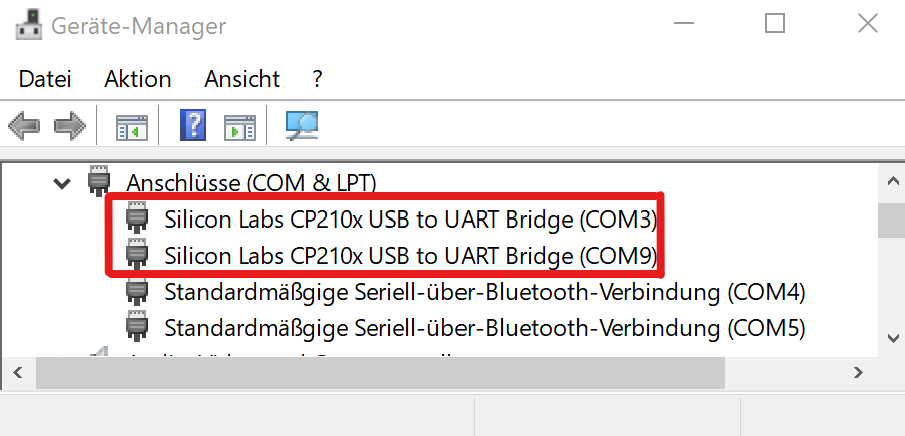
\includegraphics[width = 0.6 \textwidth]{graphics/USB_Devices_Ger_Man}
\caption{Geräte-Manager mit den aufgelisteten USB-UART-Converter (Mikrocontroller und WiFi-Modul).}
\label{fig:USB_Devices_Ger_Man}
\end{figure}

\subsection{Mikrocontroller}\label{Appendix:Handshake_uC}

\subsubsection{Wiring}\label{Appendix:Handshake_uC_wiring}

\begin{table}[H]
\center
\begin{tabular}{|c|lcl|c|}
\hline
\textbf{Mikrocontroller} & & & & \textbf{USB-Flash-Device} \\ \hline
RX & <== & direkt & === & TX  \\
TX & === & direkt & ==> & RX  \\
Reset & <== & Kondensator & === & DTR \\
\hline
\end{tabular}
\caption{Verbindung zwischen USB und Mikrocontroller.}
\label{tab:USB_uC}
\end{table}

\subsubsection{Handshake}\label{Appendix:Handshake_uc_Messung}
\begin{figure}[H]
\center
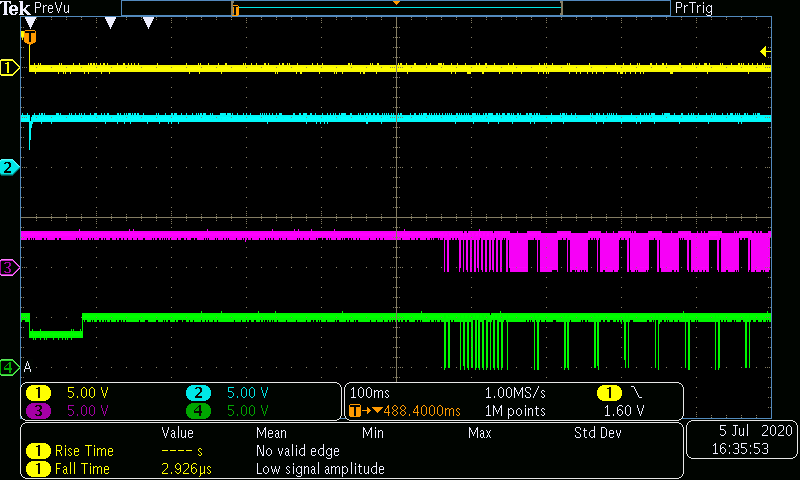
\includegraphics[width = \textwidth]{graphics/ATMega2560_DTR_RESET_RX_TX_gesamt}
\caption{Hochladen des Programmcodes auf den Mikrocontroller.\\\hspace{\textwidth}1: Gelb = DTR; 2: Blau = Reset; 3: Violett = RX; 4: Grün = TX}
\label{fig:ATMega2560_DTR_RESET_RX_TX_gesamt}
\end{figure}

\begin{figure}[H]
\center
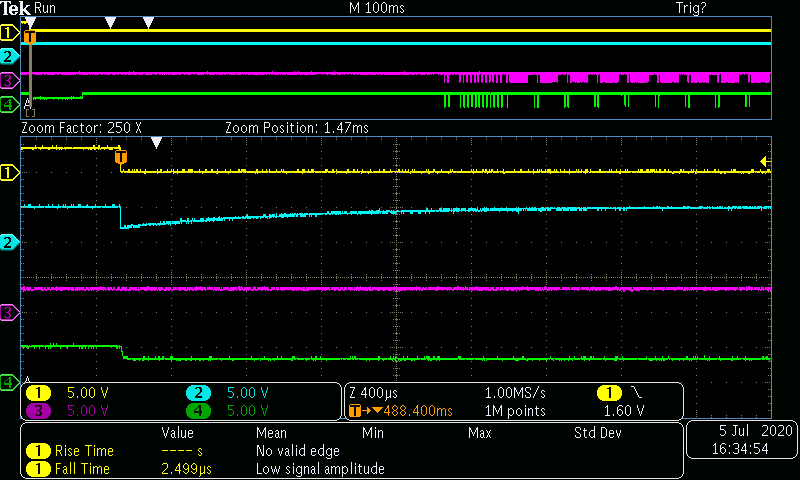
\includegraphics[width =  \textwidth]{graphics/ATMega2560_DTR_RESET_RX_TX_1}
\caption{Handshake zum Hochladen des Programmcodes auf den Mikrocontroller. Zoom auf den Moment des Resets.\\\hspace{\textwidth}1: Gelb = DTR; 2: Blau = Reset; 3: Violett = RX; 4: Grün = TX}
\label{fig:ATMega2560_DTR_RESET_RX_TX_1}
\end{figure}


\subsection{WiFi-Modul}\label{Appendix:Handshake_ESP}

\subsubsection{Wiring}\label{Appendix:Handshake_ESP_wiring}
\begin{table}[H]
\center
\begin{tabular}{|c|lcl|c|}
\hline
\textbf{WiFi-Modul} & & & & \textbf{USB-Flash-Device} \\ \hline
RX & <== & direkt & === & TX  \\
TX & === & direkt & ==> & RX  \\
EN & <== & über Transistor & === & RTS \\
IO\_0 & <== & über Transistor & === & DTR \\
IO\_13 & <== & über Widerstand & === & RTS \\
IO\_15 & <== & über Widerstand & === & CTS \\
\hline
\end{tabular}
\caption{Verbindung zwischen USB und WiFi-Modul.}
\label{tab:USB_ESP}
\end{table}

\subsubsection{Handshake}\label{Appendix:Handshake_ESP_Messung}

Im Getting Started Guide vom WiFi-Modul steht geschrieben, dass wenn während die beiden Pins IO0 und EN GND gezogen werden, das Modul in den Download-Modus versetzt wird, die Firmware über den UART-Port herunterlädt und diese in den Flash-Speicher schreibt. Um dies automatisch über die DTR- und RTS-Leitung machen zu können, braucht es eine zusätzliche Programmierlogik.

Mit der Schaltung, wie sie in Abbildung \ref{fig:Schema_ESP32_Flashbuttons} ersichtlich ist, kann das WiFi-Modul mit einer bestimmten Signalabfolge an den Leitungen DTR und RTS in diesen Download-Boot-Modus gesetzt werden. Die Auswirkung der Schaltung auf IO0 und den EN-Pin kann aus Tabelle \ref{tab:Einfluss_Boot_Schaltung} entnommen werden.

\begin{table}[H]
\center
\begin{tabular}{|c|c||c|c|}
\hline
\multicolumn{4}{|c|}{\textbf{Auto Program Cirquit}}\\
\hline
\textbf{DTR} & \textbf{RTS} & \textbf{EN} & \textbf{IO0} \\
\hline
1 & 1 & 1 & 1 \\
\hline
0 & 0 & 1 & 1 \\
\hline
1 & 0 & 0 & 1 \\
\hline
0 & 1 & 1 & 0 \\
\hline
\end{tabular}

\caption{RTS- und DTR-Signale und deren Auswirkung auf IO0 und EN.}
\label{tab:Einfluss_Boot_Schaltung}
\end{table}

Die Programmierlogik wird aus dem Programmiertool angesteuert. Es befindet sich in der Bibliothek des WiFi-Moduls, welche verwendet wird, um Code aus der Arduino-Umgebung hochzuladen. Aus dem Python-Skript kann entnommen werden, wie die Pins angesteuert werden. Der Code ist in Abbildung \ref{fig:ESP32_Boot_Code} dargestellt.\\
Bei der Interpretation des Codes ist darauf zu achten, dass die beiden Pins DTR und RTS Active-Low sind. (True = 0V = 0 = LOW und False = VCC = 1 = HIGH). Der Bezug zwischen dem Upload des Programms, den Pins des WiFi-Moduls und dessen Download-Boot-Modus sowie den Leitungen DTR und RST wird in Tabelle \ref{tab:Abfolge_Download_Boot_Modus} aufgezeigt. \cite{loboriseu_esp32_autoresetjpg_2017}
%Daraus erkennbar ist, dass:
%\begin{table}
%\begin{tabular}{lll}
%DTR & RTS & Status\\
%1 & 0 & Reset\\
%1 & 1 & Starte Run-Modus\\
%1 & 0 & IO0 = 0\\
%0 & 0 & Starte Run-Modus\\
%\hline
%\end{tabular}
%\end{table}

\begin{figure}[H]
	\centering
	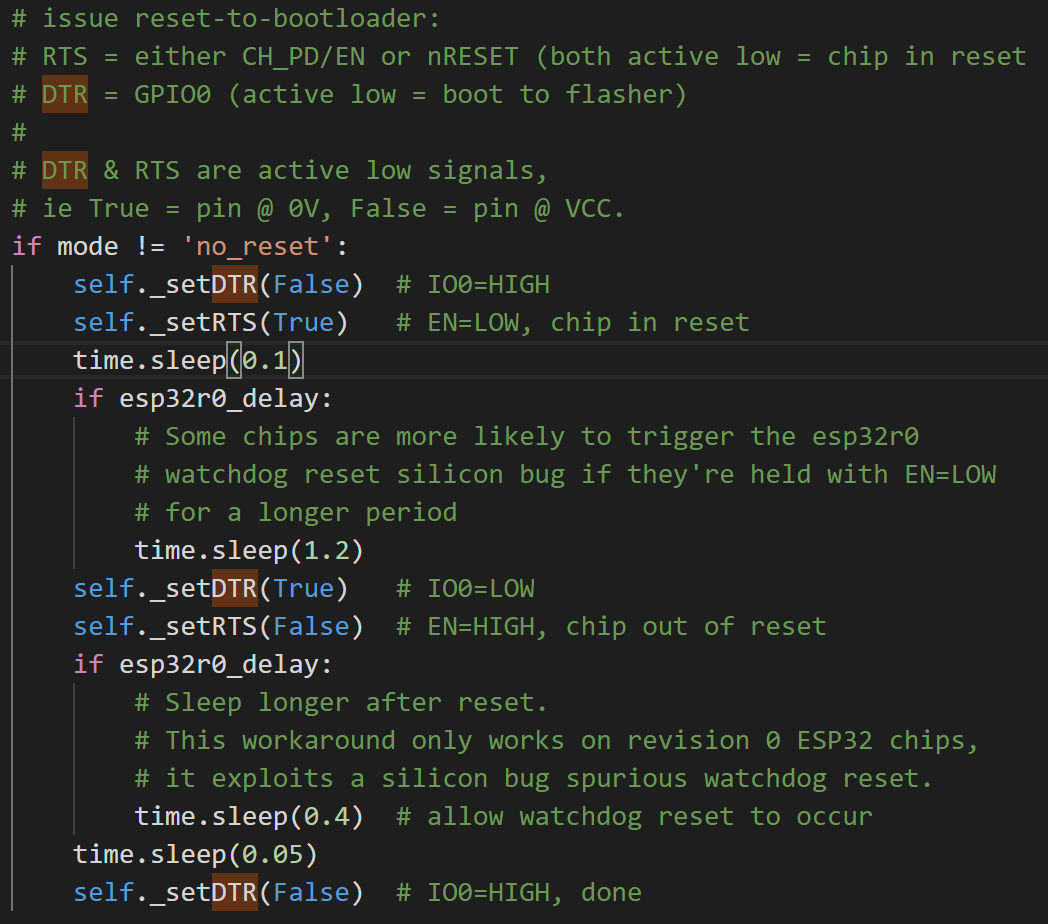
\includegraphics[width=0.8\textwidth]{graphics/ESP32_Boot_Code}
	\caption{Codeausschnitt aus dem Programmier-Tool \textit{esptool.py}. Auf diese Weise werden der DTR- und der RTS-Pin angesteuert während dem Programmiervorgang.}
	\label{fig:ESP32_Boot_Code}
\end{figure}

\begin{table}[H]
\center
\begin{tabularx}{\textwidth}{|l|X||c|c||c|c|}
\hline
Schritt & Beschreibung & DTR & RTS & EN & IO0\\
\hline
1 & Im ersten Schritt wird der Chip mit \textit{EN = 0} und \textit{IO0 = 1} in den Reset-Modus geschaltet und im Programm 0.1ms gewartet. & 1 & 0 & 0 & 1 \\
\hline
2 & Im zweiten Schritt werden die Zustände geändert, jetzt ist \textit{EN = 1} und \textit{IO0 = 0} \textit{IO0 = 0}. Aufgrund der Kapazität am EN-Pin wird die Spannung für einen kurzen Moment tief gehalten. Dies hat Schritt 3 zur Folge. & 0 & 1 & 1 & 0 \\
\hline
3 & Die durch den Kondensator C7 tief gehaltene Spannung bewirkt, dass sich die Zustsände über den Pins wie folgt verhalten: \textit{EN = 0} und \textit{IO0 = 0}. Im Programm wird 0.05ms gewartet. Danach ist das WiFi-Modul im Download-Boot-Modus und das zu speichernde Programm kann hochgeladen werden. & 0 & 1 & 0 & 0 \\
\hline
4 & Nachdem das Programm hochgeladen wurde, werden beide Zustände auf 1 gesetzt. Das WiFi-Modul startet nun den neu hochgeladenen Programmcode. & 1 & 1 & 1 & 1 \\
\hline
\end{tabularx}
\caption{Abfolge der Schritte während dem Aufrufen des Download-Boot-Modus.}
\label{tab:Abfolge_Download_Boot_Modus}
\end{table}

\begin{figure}[H]
\center
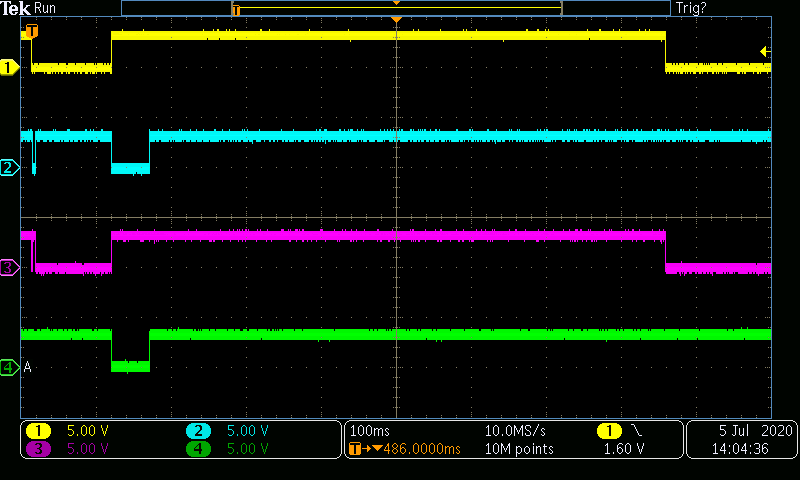
\includegraphics[width = \textwidth]{graphics/ESP32_RTS_DTR_EN_IO0_gesamt}
\caption{Handshake zum Hochladen des Programmcodes auf das WiFi-Modul. \\\hspace{\textwidth}1: Gelb = RTS; 2: Blau = DTR; 3: Violett = EN; 4: Grün = IO0;}
\label{fig:ESP32_RTS_DTR_EN_IO0_gesamt}
\end{figure}

\begin{figure}[H]
\center
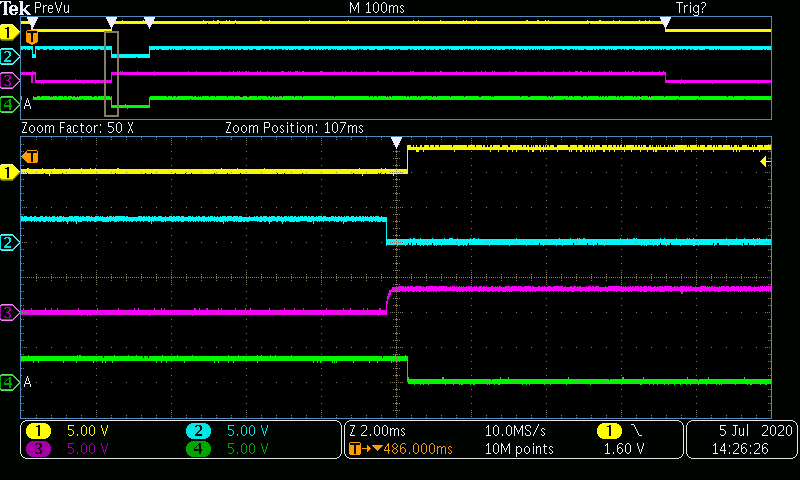
\includegraphics[width = 0.8\textwidth]{graphics/ESP32_RTS_DTR_EN_IO0_2}
\caption{Handshake zum Hochladen des Programmcodes auf das WiFi-Modul. Zoom auf gleichzeitiger Flankenwechsel RTS und DTR (Schritt 2 und 3).\\\hspace{\textwidth}1: Gelb = RTS; 2: Blau = DTR; 3: Violett = EN; 4: Grün = IO0;}
\label{fig:ESP32_RTS_DTR_EN_IO0_2}
\end{figure}


In Kapitel \ref{sec:Inbetriebnahme_Programmierschnittstellen} wurde erwähnt, dass beim Handshake die Praxis der Theorie widerspricht. Eine Recherche ergab, dass einige User zum Ergebnis kamen wie bei der Inbetriebnahme. Nämlich, dass es nach dem Reset eine Zeit dauert, bis im Startprozess die Pins geprüft werden. Dazu gehört auch der Pin IO0. Somit ist es möglich, den Pin IO0 kurz nach dem Reset auf 0 zu ziehen.
Im selben Forum wurde auch die in Abbildung \ref{fig:ESP32_Handshake_Forum} gezeigte Darstellung gefunden. Ein Kommentar weist darauf hin, das mit dem esptool.py der EN-Pin des WiFi-Moduls direkt auf RTS gehängt werden kann. So lassen sich die Zeitpunkte, zu der die Pins auf 0 sind, näher zusammenschieben. \cite{liudr_trying_2017}

Die Messung nach dem Einlöten der Brücke bestätigt dies. Abbildung \ref{fig:ESP32_RTS_DTR_EN_IO0_mit_Bruecke_1} zeigt, dass das Umschalten von EN und GPIO0 gleichzeitig passiert. Allerdings spielt der Kondensator jetzt nicht mehr so eine grosse Rolle, was auch nicht nötig ist. Auf das Hochladen des Codes hat die Brücke keinen Einfluss. Die Funktioniert wie bei der Schaltung ohne Brücke einwandfrei.


\begin{figure}[H]
\center
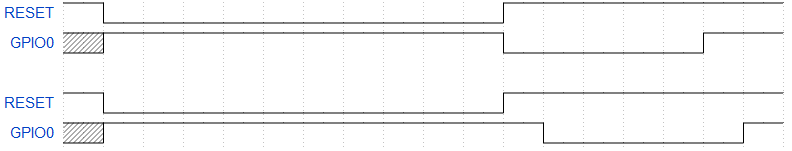
\includegraphics[width = 0.8\textwidth]{graphics/ESP32_Handshake_Forum}
\caption{Handshake zum Hochladen des Programmcodes auf das WiFi-Modul. Zoom auf gleichzeitiger Flankenwechsel RTS und DTR. \cite{liudr_trying_2017}}
\label{fig:ESP32_Handshake_Forum}
\end{figure}

\begin{figure}[H]
\center
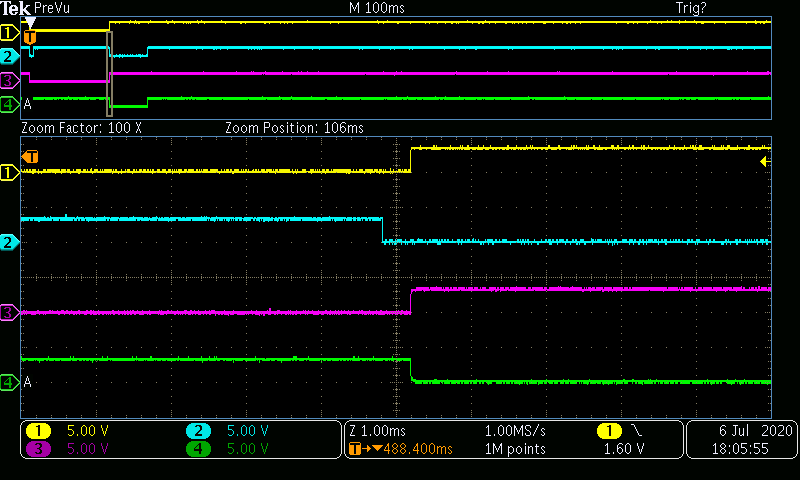
\includegraphics[width = 0.8\textwidth]{graphics/ESP32_RTS_DTR_EN_IO0_mit_Bruecke_1}
\caption{Handshake zum Hochladen des Programmcodes auf das WiFi-Modul. Zoom auf gleichzeitiger Flankenwechsel RTS und DTR.}
\label{fig:ESP32_RTS_DTR_EN_IO0_mit_Bruecke_1}
\end{figure}
